\section{Evaluation}
\label{colors:eval}

% Why and what we want to check
% How we are going to check
% Where we check it - i.e. computer

% Experimental setup:
% 1. Memory cap + stats using Cap
% 2. Using problems from cvc4 induction with aggregated proof terms
% 3. Configurations - runtime, memory 
% Problems in creating an experiment with existing systems
% Different variants being tested and implementations. Everything is based on TheSy's case split mechanism.
% 1. TheSy cloning, but keep splits to simulate memory use
% 2. TheSy with colors - no colored e-nodes
% 3. TheSy with colors and colored e-nodes, no deletion
% 4. Colors + colored e-nodes + deletion

% Results breakdown:
% 1. Graph size - nodes and memory usage
% 2. Total memory usage
% 3. Runtime

Support for colored e-graphs is implemented in
a modified version of egg, called Easter Egg.
In this section, we evaluate the performance and effectiveness of Easter Egg and the different optimizations we presented.
For this purpose we implemented two versions of colored e-graphs containing different improvements described in \autoref{colors:optimizations}.
The simple version only uses procedural improvements, while the optimized version uses all optimizations.

\subsection{Objectives and Evaluation Method}
Our evaluation aims to test colored e-graphs' efficacy in equality saturation for exploratory reasoning tasks with multiple simultaneous assumptions. 
We evaluate the effectiveness using e-graph size and equality saturation time. 
To the best of our knowledge, a purely e-graph-based automated theorem prover does not exist, and theory exploration tools have limited support for conditions.
Thus, for the evaluation, we created an equality saturation-based prover (based on code from~\cite{thesy}) that incorporates an automatic case-splitting mechanism. 

The case-splitting mechanism is only used when it will potentially contribute to progress of the equality saturation process---that is, when it enables additional rewrite rules that were previously blocked.
When this is detected, the prover yields appropriate assumptions, one for each case.
We compare two settings:
a baseline setting with separate e-graphs
created by cloning, and Easter Egg's colored e-graph implementation.
We measure the total running times and the total size of all the e-graphs.
%The comparison includes the combined size of all clones to mimic exploratory reasoning.

We evaluated our implementation on inductive proof suites from \cite{cvc4induction}, also used in \cite{thesy}. 
Since the instances are relatively small, we introduced a slight variation: for each goal, we combined benchmarks (i.e. proof goals) within the suite sharing similar goals and vocabulary.
This approach generates larger benchmarks, and thus larger e-graphs, for more significant exploration, with the prover continuing until saturation or resource limit, regardless of early goal achievement.
All the experiments were conducted on 64 core AMD EPYC 7742 processor with 512 GB RAM.

\subsection{Experimental Setup}
%In this subsection, we provide a detailed description of the experimental setup we employed to compare colored e-graphs with the baseline of using a set of separate e-graphs.

Using the enhanced prover, we evaluated each test case by measuring e-graph sizes and run times. 
E-graph size was determined by counting e-nodes; in colored layers, we tracked additional colored e-nodes, whereas for separate e-graphs, we measured the e-nodes in both the original and coarsened graphs.
The experiments utilize the Cap library to cap memory usage at 32 GB and limit run-time to 1 hour per case.

Our experiments involved a basic colored e-graph implementation (as per \autoref{colors:overview} which we dub monochrome colored e-graph, as it does not contain colored e-nodes) and a fully optimized version, comparing both against the baseline of separate e-graphs. 
The pruning optimization has almost identical results to the fully optimized version, and hence, for brevity, it is not shown. 
It is expected, due to pruning being ineffective in cases where the same rewrite rules are applied repeatedly, adding the removed e-nodes right back.


\subsection{Results}


\begin{figure*}[t]
  \raggedleft
  \newcommand\axislab[1]{\fontsize{9pt}{9pt}\selectfont{#1}}
\begin{tikzpicture}
  \node(mono)[inner sep=0,draw] {
   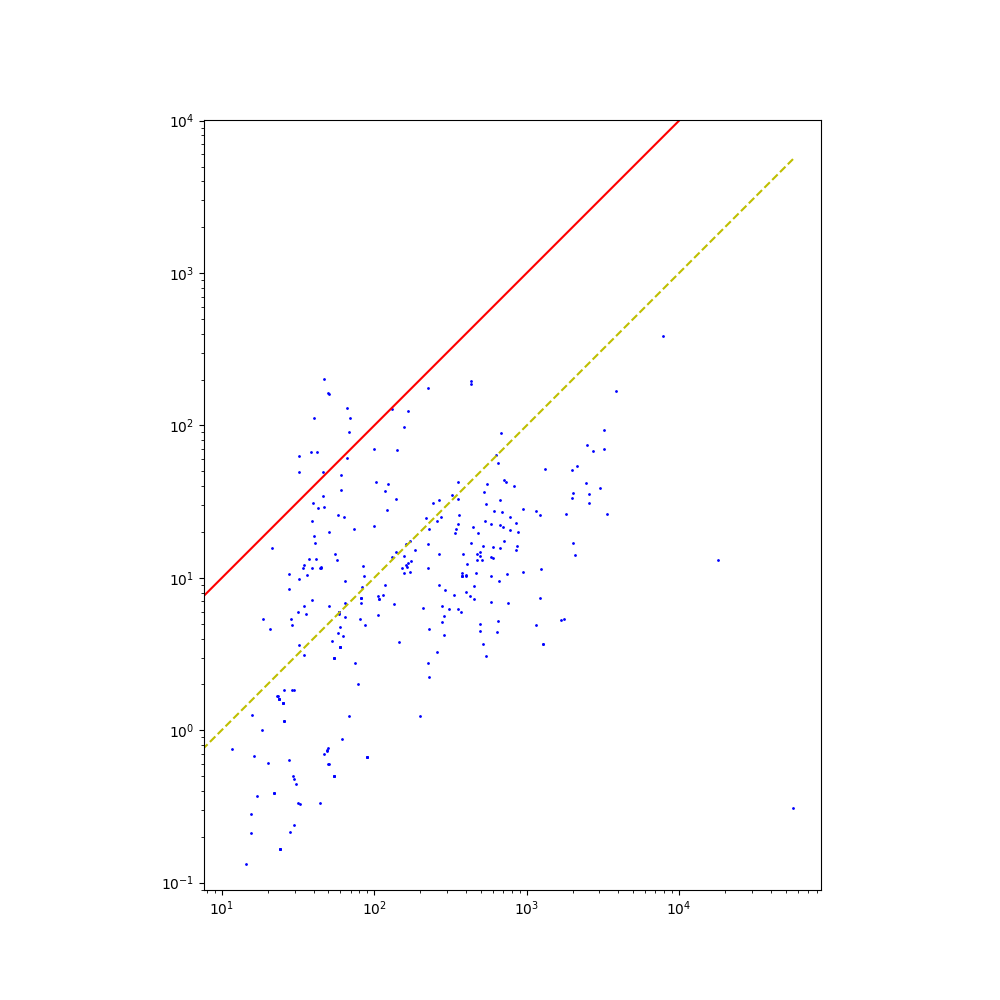
\includegraphics[width=0.35\textwidth,
                    trim=32mm 15mm 15mm 20mm] 
     {colors/gfx/normsize-no_cmemo.png}
     };
  \node(opt)[right=10mm of mono, inner sep=0] {
   \includegraphics[width=0.35\textwidth,
                    trim=32mm 15mm 20mm 20mm] 
     {colors/gfx/normsize-colored.png}
     };
  \node[below=-1mm of mono] {\axislab{separate e-graphs}};
  \node[left=-3mm of mono, rotate=90, anchor=south] {\axislab{monochrome colored e-graphs}};
  \node[below=-1mm of opt] {\axislab{separate e-graphs}};
  \node[left=-3mm of opt, rotate=90, anchor=south] {\axislab{optimized colored e-graphs}};
  \node(a)[right=10mm of opt] {$\times 1$};
  \node(b)[below=10mm of a.west,anchor=west] {$\times 10$};
  \draw[red,line width=0.8pt] (a.west) -- ++(-1, 0);
  \draw[yellow!50!gray,line width=1pt,dash pattern=on 2pt off 1pt] (b.west) -- ++(-1, 0);
\end{tikzpicture}
  %\includegraphics[width=0.3\textwidth]{gfx/normsize-colored.png}
  %\end{tabular}
  \vspace{-1em}
  \caption{Size comparison: relative e-node overhead in clones \vs color e-graph variants.}
  \label{fig:normalizedsize}
  \vspace{0.5em}
\end{figure*}

In our setup, all assumptions emerge from case splits done by the prover.
We filter out cases where no case splits were applied, since these have no assumptions introduced and thus colored e-graphs have no impact.

For each benchmark instance, we measure the \emph{relative e-node overhead} as the number of additional e-nodes that are required, normalized by the number of different assumptions.
That is, $(|\textrm{total e-nodes}| - |\textrm{base e-nodes}|) / |\textrm{assumptions}|$.
``Base e-nodes'' represent the contents of the graph before case splits.
(For the monochrome colored e-graph we use the base e-nodes present in the separate e-graphs case.)
\autoref{fig:normalizedsize} summarizes the results, pitting colored e-graphs (with and without colored e-nodes) against the baseline of separate clones.
In some cases one configuration times out or runs out of memory, while the other does not;
we only compare cases where both configurations finished the run successfully.
In both comparisons, we see roughly around 10$\times$ lower overhead, where in the monochromatic case samples are more dispersed around the y axis, and the optimized case shows clear advantage to the colored e-graph implementation.


Run-time is measured as the the total run-time for completed test cases, and 1 hour for cases that timed out.
We do not include runs that did not finish due to out-of-memory exceptions (we report the latter separately).
As can be seen in \autoref{fig:runtime}, the monochrome colored e-graph lead to many timeouts,
whereas the optimized case exhibits running times similar to separate clones.
This is in line with our expectation:
colors provide lower memory sizes at the expense of run-time.

\begin{figure*}
  \centering
  \newcommand\axislab[1]{\fontsize{7pt}{9pt}\selectfont{#1}}
\begin{tikzpicture}
  \node(mono)[inner sep=0] {
   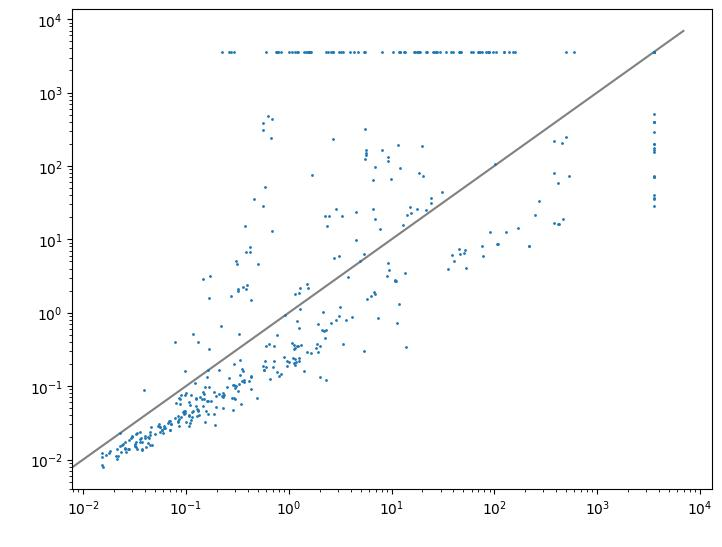
\includegraphics[width=0.35\textwidth, trim=20 20 20 15] 
     {colors/gfx/runtime-no_cmemo.jpg}
     };
  \node(opt)[right=12mm of mono, inner sep=0] {
   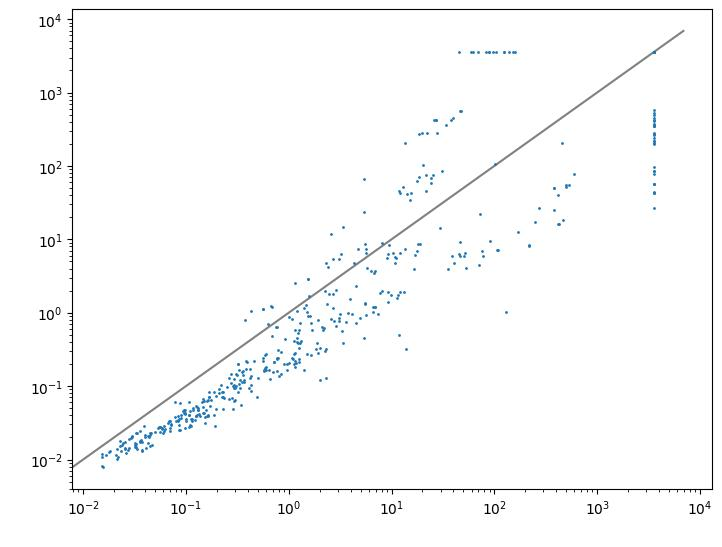
\includegraphics[width=0.35\textwidth, trim=20 20 20 15] 
     {colors/gfx/runtime-colored.jpg}
     };
  \node[below=0mm of mono] {\axislab{separate e-graphs}};
  \node[left=0mm of mono, rotate=90, anchor=south] {\axislab{monochrome colored e-graphs}};
  \node[below=0mm of opt] {\axislab{separate e-graphs}};
  \node[left=0mm of opt, rotate=90, anchor=south] {\axislab{optimized colored e-graphs}};
\end{tikzpicture}
    \vspace{-1em}
    \caption{Run-time comparison: run-time of clones vs. color e-graphs}
    \label{fig:runtime}
\end{figure*}

Finally, in \autoref{tab:runtimesuite} we present the number of out-of-memory exceptions, the number of timeout exceptions, and total run-time for each configurations and test suite.
The monochrome colored e-graph, as expected, exhibits many timeouts. 
Even though it has more errors than the other e-graph versions, it still has much longer run-times.

The optimized e-graphs demonstrate enhancements over separate e-graphs in both run-time and success rate, as detailed in \autoref{tab:runtimesuite}. 
Notably, the optimized configuration completed more tests (99 failures compared to 114). 
A key shift observed is the replacement of out-of-memory errors with timeouts, particularly in the \funcname{leon-amortize-queue} suite. 
However, \funcname{leon-heap} posed challenges for colored e-graphs, incurring 13 extra timeouts even in the optimized version. 
Conversely, the \funcname{isaplanner} suite showed a notable improvement, halving the failure rate in the optimized version compared to the baseline.

% I have a problem in how I test this, because it requires to assert both cases finished running and I can't do that at the moment
\begin{comment}
The \funcname{isaplanner} test suite contains a similar disparity, where for 79 test cases the colored e-graph has more assumptions by the end of the run.
There are no cases in \funcname{isaplanner} where the colored e-graphs had fewer assumptions, and there are only 4 test cases for which colored e-graphs had more assumptions in \funcname{leon-heap}, and none in which it had fewer.
\end{comment}


\begin{table}[t]
    \centering
    \caption{Run-time and exceptions. M = Out of memory, T = Timeout (3600) }
    \label{tab:runtimesuite}
    \setlength{\tabcolsep}{3pt} % Adjust the space between columns
    \newcolumntype{d}[1]{D{/}{/}{#1}} % New column type for O/T column
    \begin{tabular}{lrd{3}rd{3}rd{3}}
    \toprule
    & \multicolumn{2}{c}{Separate} & \multicolumn{2}{c}{Monochrome} & \multicolumn{2}{c}{Optimized} \\
    \cmidrule(r){2-3} \cmidrule(lr){4-5} \cmidrule(l){6-7}
    Test Suite & \multicolumn{1}{c}{Time} & \multicolumn{1}{l}{M/T} & \multicolumn{1}{r}{Time} & \multicolumn{1}{l}{M/T} & \multicolumn{1}{r}{Time} & \multicolumn{1}{l}{M/T} \\
    \midrule
    clam & 70.1 & 0/0 & 277.8 & 0/5 & 23.6 & 0/0 \\
    hipspec-rev-equiv & 34.1 & 0/0 & 139.0 & 0/17 & 57.0 & 0/0 \\
    hipspec-rotate & 3880.3 & 1/1 & 1871.4 & 0/6 & 17.4 & 0/3 \\
    isaplanner & 8454.4 & 0/60 & 6068.4 & 0/70 & 20486.3 & 3/28 \\
    leon-amortize-queue & 187356.4 & 52/0 & 14.8 & 0/57 & 10854.3 & 3/49 \\
    leon-heap & 1735.9 & 0/0 & 1201.8 & 0/25 & 4949.2 & 0/13 \\
    \bottomrule
    \end{tabular}
\end{table}







\begin{comment}
    \begin{tabular}{llr}
\toprule
 &  & Time \\
E-graph Type & Test Suite &  \\
\midrule
\multirow[t]{7}{*}{Seperate e-graphs} & clam & 34.234764 \\
 & hipspec-nichomachus & 0.050861 \\
 & hipspec-rev-equiv & 2.577174 \\
 & hipspec-rotate & 237.717540 \\
 & isaplanner & 8913.695004 \\
 & leon-amortize-queue & 9.668328 \\
 & leon-heap & 216.857437 \\
\cline{1-3}
\multirow[t]{7}{*}{Monochromatic colored e-graphs} & clam & 394.891332 \\
 & hipspec-nichomachus & 0.087772 \\
 & hipspec-rev-equiv & 0.720120 \\
 & hipspec-rotate & 1970.451256 \\
 & isaplanner & 1739.190107 \\
 & leon-amortize-queue & 0.294397 \\
 & leon-heap & 1206.035020 \\
\cline{1-3}
\multirow[t]{7}{*}{Optimized colored e-graphs} & clam & 6.049511 \\
 & hipspec-nichomachus & 0.085397 \\
 & hipspec-rev-equiv & 42.016671 \\
 & hipspec-rotate & 78.174158 \\
 & isaplanner & 12337.053032 \\
 & leon-amortize-queue & 43.787478 \\
 & leon-heap & 791.375722 \\
\cline{1-3}
\bottomrule
\end{tabular}
\end{comment}